\section{Introduction}

The Gut-microbiome is by far the best and widely studied microbial ecosystem of the human anatomy, partly due to the rich microbial environment and partly due to the ease of sample collection (non-invasive) through faeces \cite{Budden2017}. On the other hand, the healthy lung was long considered to be sterile, but with advent high-throughput sequencing techniques, this has been proven otherwise \cite{Barker2002}. Extensive research on the gut-microbiota has that shown that gut microbiota is capable of influencing other organs, such as the brain, liver or lungs \cite{Bell2019}. This has led to the coining of terms such as the `gut-brain axis' and the `lung-gut axis'. 

Growth of pathogenic microbes in the lung can cause diseases such as \emph{Nontuberculous mycobacteria} (NTM) infections. NTMs are mycobacteria other than \emph{M. tuberculosis} (the cause of tuberculosis) and \emph{M. leprae} (the cause of leprosy). Although anyone can get an NTM infection, NTM are opportunistic pathogens and hence most commonly affects people with an underlying lung disease such as chronic obstructive pulmonary disease (COPD), bronchiectasis, cystic fibrosis and primary ciliary dyskinesia. The most common symptoms include a persistent cough, fatigue, weight loss, night sweats, and occasionally shortness of breath (dyspnoea) and coughing up of blood (haemoptysis)\cite{Ratnatunga2020}.

The epithelial surfaces of the gut and lung are exposed to diverse microbes; ingested microorganisms can access both sites, and the microbiota from the gut can enter the lungs through processes such as micro-aspiration \cite{Budden2017}. Furthermore, the lung and gut can interact thorough the systemic cytokines released by host immune cells in response to microbes or microbes from one-site may secrete metabolites which are absorbed into the bloodstream and thus regulate the organs \cite{Dang2019}. A study used germ-free mice, which lack an appropriately developed immune system and showed mucosal alterations, both of which is restored through colonization with gut microbiota. Thus, supplementing the concept of `lung-gut' axis \cite{Budden2017}.

Literature survey using the keyword `lung-gut axis' shows that this concept was first introduced in 2014 and is gaining popularity with increasing work being done \ref{ch2_fig1}. Although this hypothesised concept is gaining popularity and increasingly believed, it has not been proven experimentally using interventional studies and it`s role in diseases not well characterised. This increasing evidence also suggests, a potential existence of lung-gut axis and its effectual role in lung diseases. The lung-gut axis is only beginning to be understood; emerging evidence indicates that there is potential for manipulation of the gut microbiota in the treatment of lung diseases. Despite this, the influence of microbial gut health in Bronchiectasis lung is poorly studied. 

Bronchiectasis is a chronic inflammatory respiratory disease associated with progressive, irreversible dilatation of the airway. Exacerbation in bronchiectasis is defined as the acute episode of progressive worsening of symptoms including shortness of breath and cough. It is crucial to study bronchiectasis because in most cases it is known to be idiopathic(unknown cause) \cite{pmid29478908} and it is a significant contributor to lung diseases globally with a substantial four-fold higher predominance in Asian populations \cite{Seitz2012}. Hence, in the second chapter of my PhD thesis, I would like to study the effect of lung-gut axis in bronchiectasis. I largely plan to do this using the integrative tools I developed in my previous chapter. Moreover, Chapter1 of my thesis focused on integrating multiple microbiomes from the same site (i.e. the lung) here I plan on extending this to integrating multiple microbiomes from multiple site (i.e. lung and gut). 

\begin{figure}[ht]
	\centering
	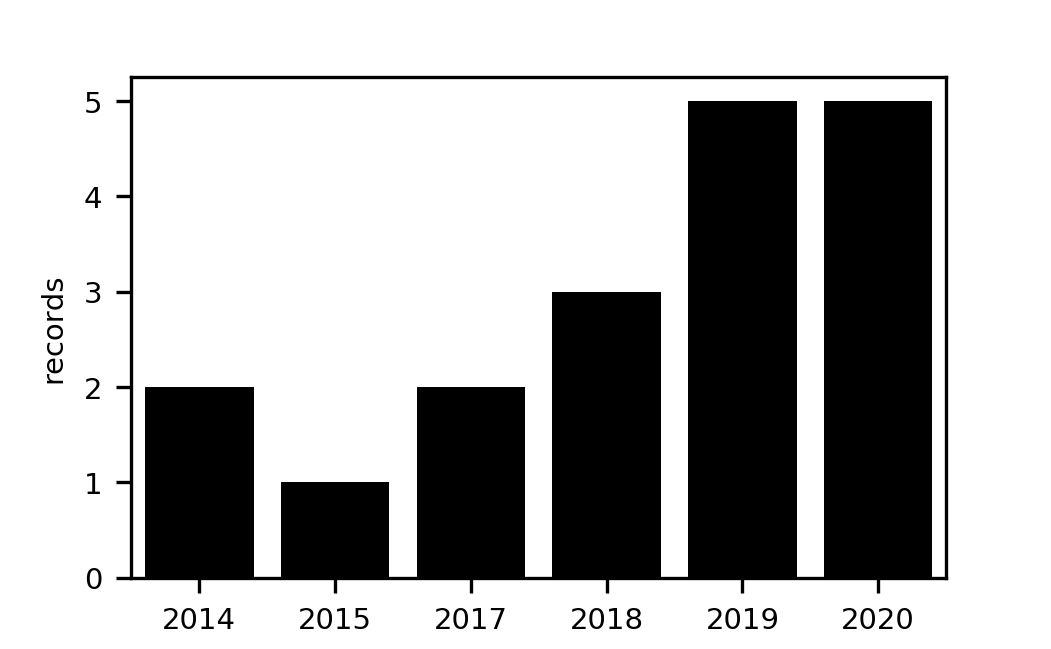
\includegraphics[width=0.5\textwidth]{./image/bar-papers.png}
	\caption{A histogram illustrating all available publications (including original articles and perspectives) matching the keyword ``lung-gut axis" from 1900 to 2020 in the web of science database.}
	\label{ch2_fig1}
\end{figure}